%% Week 37 -- Tuesday session (flipped classroom)
%% Companion to week37slides.tex (Monday lecture).  Two cases only, by
%% design, and no warm-up frames: the first twenty minutes are open questions
%% from Monday.  Case 1 = your own gradient descent for OLS and Ridge with
%% analytical gradients on the week-37 exercise data (scaling, gradients,
%% closed form, learning rate, stopping, the eigenvalue bound) -- this is
%% exercises 1-4 of the week and part e) of Project 1.  Case 2 = momentum and
%% the JAX gradient on the Runge function of Project 1 (parts e and f), with
%% the finite-difference check.  Each case is followed by an "insight
%% questions" frame (3-4 questions, answers on \pause) for the plenary; the
%% same questions sit in the notebook and, with the answers as a self-check
%% table, at the end of exercisesweek37.ipynb.  The cases are worked in
%% week37tuesday.ipynb.
%% Build:  pdflatex week37tuesday.tex  (twice)
\documentclass[10pt,aspectratio=169]{beamer}
\usetheme{red_plain}
\usepackage[T1]{fontenc}
\usepackage[utf8]{inputenc}
\usepackage{amsmath,amssymb,bm}
\usepackage{graphicx}
\usepackage{listings}
\usepackage{xcolor}
\usepackage{booktabs}
\graphicspath{{../BookFigures/chapter04_optimization/}{./}}

%% ---- code listings
\definecolor{codebg}{rgb}{0.97,0.97,0.97}
\lstset{language=Python,basicstyle=\ttfamily\scriptsize,backgroundcolor=\color{codebg},
  keywordstyle=\color{blue!70!black}\bfseries,commentstyle=\color{green!45!black},
  stringstyle=\color{red!60!black},showstringspaces=false,frame=single,
  framerule=0pt,xleftmargin=4pt,xrightmargin=4pt,breaklines=true,columns=fullflexible}

%% ---- discussion frames (same machinery as the Monday "Pause and think";
%% kept for future weeks, unused in this deck since the warm-ups were dropped)
\newcounter{insight}
\newenvironment{insight}[1][]{%
  \stepcounter{insight}%
  \begin{frame}{Warm-up \arabic{insight}: #1}%
  \setbeamercolor{block title}{bg=structure.fg,fg=white}%
  \setbeamercolor{block body}{bg=structure.fg!8}%
}{\end{frame}}
\newcommand{\question}[1]{\begin{block}{Question}#1\end{block}}
\newcommand{\answer}[1]{\pause\begin{block}{Answer}#1\end{block}}
\newcommand{\hint}[1]{\pause{\small\emph{Hint: }#1}}

%% ---- case frames
\newcounter{case}
\newenvironment{case}[1][]{%
  \stepcounter{case}%
  \begin{frame}[fragile,environment=case]{Case \arabic{case}: #1}%
}{\end{frame}}

\setbeamertemplate{footline}[frame number]
\setbeamertemplate{blocks}[rounded][shadow=false]
\setbeamercovered{invisible}

\title{Week 37, Tuesday Session}
\subtitle{Flipped classroom: your questions, then gradient descent in practice\\[3pt]
  \small Bring your laptop -- we work in \texttt{week37tuesday.ipynb}}
\author{Morten Hjorth-Jensen}
\institute{Department of Physics and Center for Computing in Science Education,\\
  University of Oslo, Norway}
\date{}

\begin{document}

\begin{frame}
\titlepage
\end{frame}

\begin{frame}{How today works}
\begin{block}{The format (as every Tuesday)}
Mondays are lectures; Tuesdays belong to your questions and to concrete
cases.  You have heard the lecture and skimmed Sections 3.14, 4.1--4.6 and
4.14.
\end{block}
\begin{enumerate}
  \item \textbf{First $\sim$20 min:} your open questions from Monday's
        lecture and from the reading, discussed in plenum.  Cross-validation
        questions are welcome here too -- Project 1 part d) is still open.
  \item \textbf{Rest of the double session:} \emph{two} cases only --
        your own gradient descent code for OLS and Ridge with analytical
        gradients, and momentum plus the automatic gradient on the Runge
        function -- worked in pairs or small groups from
        \texttt{week37tuesday.ipynb}.  Deep beats broad: the goal is that
        you leave with a working, \emph{checked} gradient descent code and
        an understanding of what the learning rate can and cannot be.  Case 1
        is this week's exercises; Cases 1 and 2 together are parts e) and
        f) of Project 1.
  \item \textbf{Last 5 min:} wrap-up, exercise deadline, and what next Monday
        builds on.
\end{enumerate}
\end{frame}

\begin{frame}{Picking up from Monday: the learning rate is a property of the data}
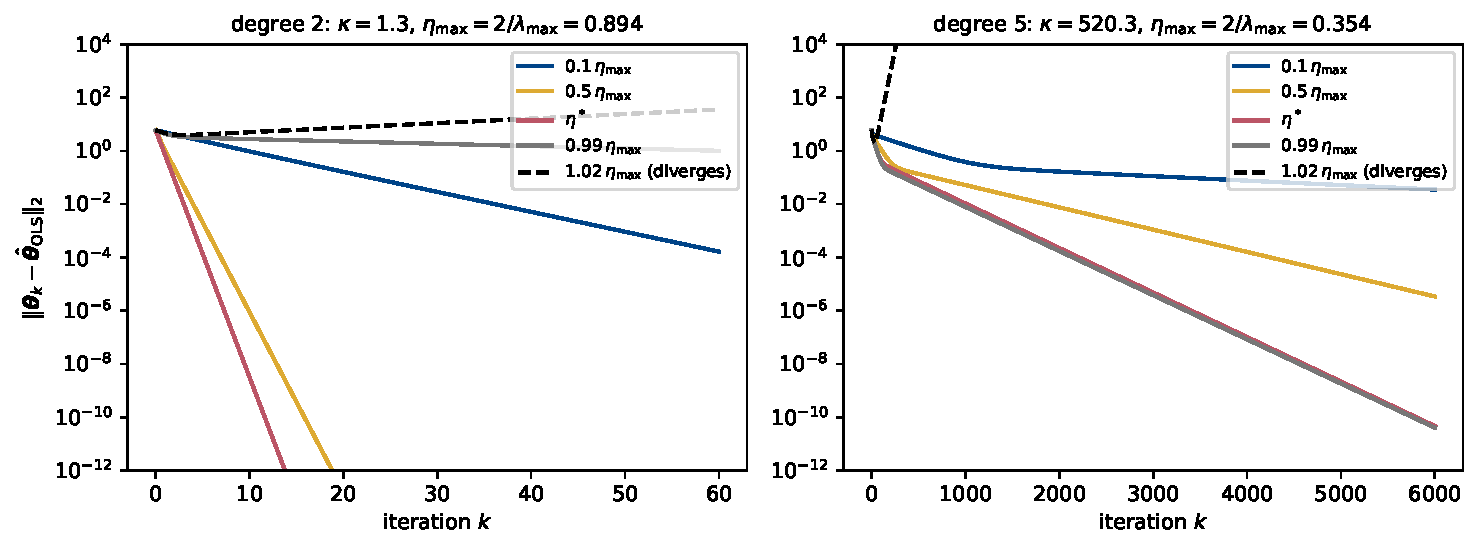
\includegraphics[width=0.98\textwidth]{week37_gd_convergence}
\vspace{1pt}
\small
Monday's central result, Eq.~(4.19): along each eigendirection of the
Hessian the error contracts by $|1-\eta\lambda_i|$ per step, so the iteration
is stable iff $\eta<2/\lambda_{\max}$ and needs $\propto\kappa$ iterations.
\textbf{Left:} degree 2, $\kappa=1.3$, 11 iterations at $\eta^*$.
\textbf{Right:} degree 5 on the same data, $\kappa=520$, 4964 iterations at
$\eta^*$ -- and $\eta_{\max}$ has moved from $0.89$ to $0.35$.  Today you
build the code that produced this figure, check the bound on \emph{your}
Hessian, and then make the slow case fast with momentum.
\end{frame}

\begin{case}[your own gradient descent for OLS and Ridge, checked]
\small
\textbf{Goal:} exercises 1--4 of this week, done together (notebook, Case 1;
seed 2026 gives exactly the lecture numbers).  Data $f(x)=2-x+5x^2$ on
$[-2,2]$, $n=100$, noise $\sigma=0.5$.
\begin{enumerate}
  \item \textbf{Scale} (exercise 1): standardise the columns of the
        polynomial design matrix, centre $\bm{y}$, no intercept column.  Why
        does centring $\bm{y}$ let us drop the intercept?
  \item \textbf{Gradients and Hessian} (exercise 2): write
        \texttt{gradient(theta, X, y, lam)} from Eqs.~(4.13) and (4.17), and
        \texttt{hessian\_eigs}.  Check the gradient at a random
        $\bm{\theta}$ against a central difference, $h=10^{-5}$ (agreement
        $\sim10^{-9}$, not $10^{-15}$: Case 2 says why).
  \item \textbf{Closed forms} (exercise 3): OLS and Ridge with the
        $n\lambda\bm{I}$ of Eq.~(3.95).  Compare with
        \texttt{Ridge(alpha=n*lam)}.
  \item \textbf{Gradient descent} (exercise 4): the loop of Eq.~(4.15) with
        a stopping criterion on $\|\nabla C\|$.  Degree 2: run
        $\eta\in\{0.01,0.1,0.5,0.8\}$; then degree 5 with the same values.
        What happens at $0.5$ and $0.8$ for degree 5, and why?
  \item \textbf{The bound:} compute $\lambda_{\max},\lambda_{\min}$ of the
        Hessian, hence $\eta_{\max}=2/\lambda_{\max}$ and
        $\eta^*=2/(\lambda_{\max}+\lambda_{\min})$; run at $0.99\,\eta_{\max}$
        and $1.02\,\eta_{\max}$.  Then Ridge with $\lambda\in\{10^{-2},10^{-1}\}$:
        what does the penalty do to $\kappa$ and to the iteration count?
\end{enumerate}
\vspace{1pt}
\begin{block}{Checkpoints (plenary after $\sim$30 min)}
Degree 2: $\hat{\bm{\theta}}=(-1.077,\,5.855)$, $\kappa=1.3$, $\eta^*=0.5$,
11 iterations.  Degree 5: $\kappa=520$, $\eta_{\max}=0.354$, $\eta^*$ needs
4964 iterations, $\eta=0.1$ needs 11\,836; Ridge $\lambda=0.1$ brings
$\kappa$ to 28.
\end{block}
\end{case}

\begin{frame}[fragile]{Case 1: the code you should end up with}
\begin{lstlisting}
def gradient(theta, X, y, lam=0.0):
    """Eqs. (4.13) and (4.17): gradient of (1/n)||X theta - y||^2 + lam theta^T theta."""
    n = len(y)
    return (2.0 / n) * X.T @ (X @ theta - y) + 2.0 * lam * theta

def gradient_descent(X, y, eta, lam=0.0, num_iters=1000, tol=1e-8, theta0=None):
    """Plain gradient descent, Eq. (4.15). Returns the iterates and the number of steps."""
    p = X.shape[1]
    theta = np.zeros(p) if theta0 is None else theta0.copy()
    history = [theta.copy()]
    for t in range(num_iters):
        g = gradient(theta, X, y, lam)
        theta = theta - eta * g
        history.append(theta.copy())
        if np.linalg.norm(g) < tol:
            break
    return np.array(history), t + 1

def hessian_eigs(X, lam=0.0):
    """Eigenvalues of the Hessian (2/n) X^T X + 2 lambda I, Eqs. (4.14) and (4.17)."""
    n = len(X)
    return np.linalg.eigvalsh((2.0 / n) * X.T @ X + 2.0 * lam * np.eye(X.shape[1]))
\end{lstlisting}
\footnotesize
Three functions, each doing one thing: \texttt{gradient} is the only place
the cost enters; \texttt{gradient\_descent} is joined by
\texttt{momentum\_descent} today and by the adaptive methods next week.
Keep the \texttt{history}: it is what you plot.
\end{frame}

\begin{frame}{Case 1: do you have the insight?  (plenary, $\sim$5 min)}
\small
\begin{enumerate}
  \item Your loop stopped after its 1000 allowed iterations with
        $\|\nabla C\|=10^{-4}$, small but not below tolerance.  Has it
        converged?  What single number tells you how far off you may still be?
  \item Standardising the columns changed the iteration count by two orders
        of magnitude but not the fitted curve.  Why does gradient descent care
        about the scaling when the closed form does not?
  \item Ridge with $\lambda=0.1$ converged in a twentieth of the iterations
        OLS needed.  Is the point it converged to a better solution of the
        OLS problem?
  \item The same code diverged at $\eta=0.5$ on degree 5 and converged at
        $\eta=0.8$ on degree 2.  Where does the boundary come from, and what
        should the code compute before it starts?
\end{enumerate}
\pause
\begin{block}{What we hope you say}
\footnotesize
(1) No.  The slow direction contracts by $|1-\eta\lambda_{\min}|$ per step;
the residual error is $\|\nabla C\|/\lambda_{\min}$ at worst -- with
$\lambda_{\min}=0.011$ that is $10^{-2}$ in $\bm{\theta}$, the second decimal.
Stop on the gradient, not on a count.
(2) The closed form solves the normal equations in one go, whatever the
units; gradient descent takes the \emph{same} step in every direction, and
the columns' scales set the eigenvalue spread $\kappa$, Eq.~(4.22), hence the
iteration count.  Same minimum, different road.
(3) No -- it is the exact solution of a \emph{different} problem, Eq.~(4.16).
The penalty lifts $\lambda_{\min}$, Eq.~(4.17), so the road gets shorter, but
the destination moved: bias for variance, Section~3.8.
(4) $\eta<2/\lambda_{\max}$, Eq.~(4.20); $\lambda_{\max}$ is a property of
$\bm{X}$, not of the algorithm.  One line: \texttt{eigvalsh(2/n X.T@X).max()}.
\end{block}
\end{frame}

\begin{case}[momentum and the automatic gradient on the Runge function]
\textbf{Goal:} parts e) and f) of Project 1 in miniature (notebook, Case 2).
Data $f(x)=1/(1+25x^2)$ on $[-1,1]$, $n=100$, $\sigma=0.1$, degree 6,
standardised columns, centred $\bm{y}$.
\begin{enumerate}
  \item \textbf{The gradient without deriving it:} write the OLS and Ridge
        costs as ordinary functions of $\bm{\theta}$, obtain
        \texttt{jax.grad} of each, and compare with your \texttt{gradient}
        from Case 1 at a random $\bm{\theta}$.  Agreement to $10^{-15}$ --
        and only to $10^{-6}$ if you forget \texttt{jax\_enable\_x64}.
  \item \textbf{Finite differences against AD:} the error of the central
        difference of one component against $h$ from $10^{-13}$ to $10^{-1}$
        (reproduce panel (b) of \texttt{week37\_ad\_check.pdf}).  Then the
        same for $f(x)=\sin(2\pi x+x^2)$ at $x=1$ (panel (a)).  Why do the
        two panels differ on the right?
  \item \textbf{Momentum:} add \texttt{momentum\_descent}, Eq.~(4.23) -- one
        line more than Case 1.  At $\eta=0.9\cdot2/\lambda_{\max}$ run
        $\gamma\in\{0,0.5,0.9\}$ and count the iterations to
        $\|\bm{\theta}_k-\hat{\bm{\theta}}\|<10^{-6}$.  Reproduce
        \texttt{week37\_momentum.pdf}.
  \item \textbf{Sensitivity to $\eta$:} repeat step 3 at $\eta_{\max}/4$ and
        at $1.5\,\eta_{\max}$.  Does momentum change where the iteration
        diverges?  (Section 4.6: stable iff $\eta\lambda_{\max}<2(1+\gamma)$.)
  \item \textbf{Swap the gradient:} run momentum with the JAX gradient
        instead of the analytical one -- the update rule does not care.
        Then \textbf{degree 10}: what is $\kappa$, and does anything converge?
\end{enumerate}
\end{case}

\begin{frame}{Case 2: what you should find}
\begin{columns}
\begin{column}{0.36\textwidth}
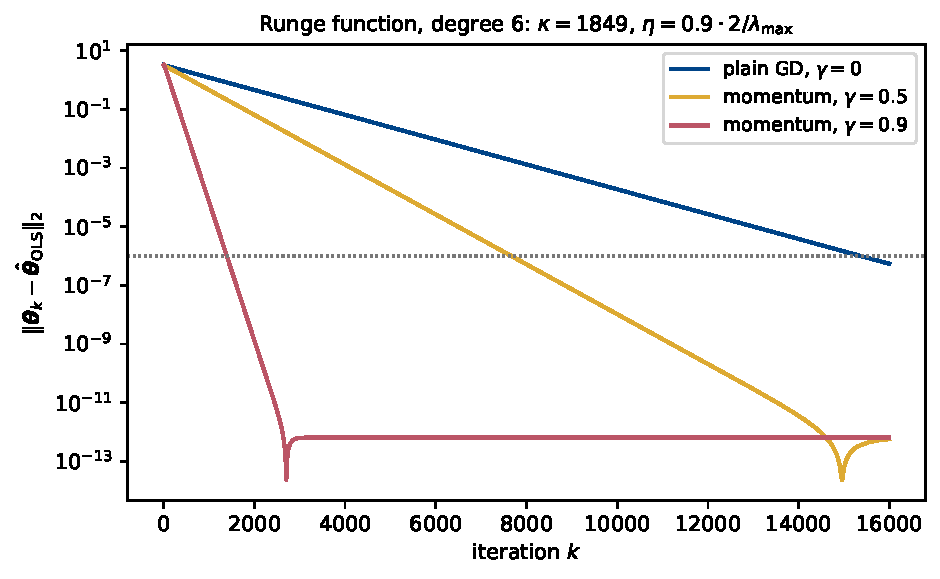
\includegraphics[width=\textwidth]{week37_momentum}
\end{column}
\begin{column}{0.62\textwidth}
\footnotesize
\begin{block}{Checkpoints (seed 2026)}
\begin{itemize}
  \item \texttt{max|AD - hand|} $=1.8\times10^{-15}$ for OLS, same order
        for Ridge.
  \item Panel (b) has no rising branch: the OLS cost is quadratic, so the
        central difference has no truncation error and only the $1/h$
        rounding error is left.  Panel (a) is the general case: best
        $10^{-11}$ at $h\approx10^{-6}$.
  \item Degree 6: $\kappa=1849$.  Iterations to $10^{-6}$: plain
        $15\,374$; $\gamma=0.5$: $7\,669$; $\gamma=0.9$: $1\,391$ -- a factor
        11, against the $\sqrt\kappa=43$ ceiling of Eq.~(4.26).
  \item At $1.5\,\eta_{\max}$ plain gradient descent diverges, $\gamma=0.5$
        sits exactly on its stability edge $2(1+\gamma)/\lambda_{\max}$ and
        oscillates for ever, and $\gamma=0.9$ converges in $761$ iterations
        -- \emph{faster} than at $0.9\,\eta_{\max}$.
  \item Degree 10: $\kappa\approx2\times10^6$; nothing converges in
        $10^5$ iterations, $\gamma=0.9$ included.  This is where week 38 --
        and Newton's method with the JAX Hessian, one step -- comes in.
        \textbf{Plenary:} with Ridge, $\lambda=10^{-3}$, momentum converges
        at degree 10 in about $3\,100$ steps ($\kappa$ drops to $5\,000$).
        Is that cheating?
\end{itemize}
\end{block}
\end{column}
\end{columns}
\end{frame}

\begin{frame}{Case 2: do you have the insight?  (plenary, $\sim$5 min)}
\small
\begin{enumerate}
  \item Your JAX gradient and your analytical gradient agree to $10^{-15}$.
        What has that proved -- and what has it \emph{not} proved?
  \item Momentum with $\gamma=0.9$ converged at $1.5\,\eta_{\max}$, where plain
        gradient descent diverged.  Does momentum make the learning rate
        unimportant?
  \item You replace the OLS cost by the cost of a neural network with $10^6$
        parameters and keep \texttt{jax.grad} and \texttt{momentum\_descent}.
        What changes in the \emph{code}?  What changes in the \emph{theory}
        you relied on today?
  \item Why is reverse mode the right mode for that network, and what does it
        cost that forward mode does not?
\end{enumerate}
\pause
\begin{block}{What we hope you say}
\footnotesize
(1) That your derivation of Eq.~(4.13) matches the cost you \emph{wrote
down} -- an error in the algebra would show up as $10^{-2}$, not $10^{-15}$.
It cannot tell you the cost itself is the one you meant (a missing $1/n$, a
penalised intercept): both gradients would agree, and both would be wrong.
(2) No.  The stability edge moved from $2/\lambda_{\max}$ to
$2(1+\gamma)/\lambda_{\max}$, and the best $\gamma$ is tied to $\kappa$,
Eq.~(4.26); $\gamma=0.5$ sat exactly on its edge and never converged.  Two
knobs instead of one, both data-dependent.
(3) Code: the definition of the cost, nothing else -- the point of AD and of
the three-function structure.  Theory: convexity is gone, so ``stationary
point = global minimum'' (Section~4.1) no longer holds and Eq.~(4.20) is only
local.  Empirical good behaviour, not a theorem.
(4) One output, $10^{6}$ inputs: reverse mode gives the whole gradient for
two or three cost evaluations, forward mode needs $10^{6}$ sweeps
(Sections~4.14.4--4.14.5).  The price is the tape -- memory, not time.
\end{block}
\end{frame}

\begin{frame}{Wrap-up, deadlines, and Monday}
\begin{itemize}
  \item \textbf{What you should own now:} a gradient descent code with a
        stopping criterion that is \emph{checked} three ways -- against the
        closed form, against a finite difference, against \texttt{jax.grad};
        the rule $\eta<2/\lambda_{\max}$ and the habit of computing
        $\lambda_{\max}$; momentum as one extra line; and one sentence on
        what automatic differentiation is not (symbolic, numerical) and what
        it costs (two or three function evaluations, whatever $p$).
  \item \textbf{Weekly exercises} (\texttt{exercisesweek37.ipynb}): Case 1
        as a write-up, plus the sparse ten-feature data set of exercise 5 and
        momentum in exercise 6.  Deadline \textbf{Friday September 11 at
        midnight}.
  \item \textbf{Project 1}, parts e) and f), ask for exactly today's
        machinery on the Runge function; part f) continues next week with
        AdaGrad, RMSProp and Adam.  The code you wrote today is directly
        reusable -- keep the three-function structure.
  \item \textbf{Next Monday (week 38):} stochastic gradient descent and the
        adaptive learning rates AdaGrad, RMSProp and Adam (Sections
        4.7--4.12), applied to Lasso (Project 1, parts g and h) and to
        logistic regression (Chapter 5).
\end{itemize}
\begin{block}{Before you leave}
One line in an email to us: the muddiest point of the week -- what should
Monday's first ten minutes revisit?
\end{block}
\end{frame}

\end{document}
